\section{Entropy and Mutual information}
\subsection{Definitions and Conventions}

\begin{definition}
    Let $(\Omega, \mathcal{A}, \mathds{P})$ be a probability space, let $\mathcal{X}$ be a countable set and
    let $X: \Omega \rightarrow \mathcal{X}$ be a discrete random variable on $(\Omega, \mathcal{A}, \mathds{P})$.
    We can then define
    \begin{align*}
        \textbf{Entropy wrt. base:}       &\quad H_b(X) = \mathbb{E}\paren{-\log_b p_X(X)} = -\sum_{x \in \supp(X)}{p_X(x) \log_b p_X(x)} \\
        \textbf{Entropy conventionally:}  &\quad H(X) = H_2(X)
    \end{align*}
\end{definition}

\begin{remark}
    \begin{enumerate}
    \item
        Let $\mathcal{X}, \mathcal{Y}$ be countable sets and $X: \Omega \rightarrow \mathcal{X}$, $Y: \Omega \rightarrow \mathcal{Y}$ 
        be discrete random variables on $(\Omega, \mathcal{A}, \mathds{P})$.
        From now on, the random variables $X, Y$ are always available for use.

    \item
        We do \textbf{not} use the shorthand notations $p(x) = \mathds{P}[X = x]$ and $p(y) = \mathds{P}[Y = y]$
        from \cite{Thomas:ElementsOfInformationTheory}, to keep the notation easily understandable.

    \item We use the convention $\log = \log_2$, as the entropy $H$ is defined wrt. base $2$.

    \item We also use the following convention and justify it through a continuity argument:
        \begin{align*}
            0 \log 0 = \lim_{x \to 0^+}{x \log x}
            = \lim_{x \to 0^+}\frac{\log x}{\frac{1}{x}}
            = \lim_{x \to 0^+}\frac{\frac{1}{\ln(2) x}}{-\frac{1}{x^2}}
            = \lim_{x \to 0^+}\frac{-x}{\ln(2)} = 0
        \end{align*}
        This choice is sensible, as $\log x$ is not defined for negative $x$.
    
        \item The conventions, definitions and theorems are from Definitions, Theorems, Remarks and Exercises 
        in \textit{Elements of Information Theory, second edition} (see \cite{Thomas:ElementsOfInformationTheory}).
    \end{enumerate}
\end{remark}

\begin{remark}[Existence of Entropy]
    Note that if $|\mathcal{X}|$ is finite, $(\forall p \in \mathbb{R}_+: H_b(X) \; \text{finite})$
    and $H(X) \le |\mathcal{X}|$ (see Theorem \ref{theorem:more-entropy-observations}).
    For $|\mathcal{X}|$ countably infinite, there are counterexamples where $H_b(X) = \infty$ (see \cite{MathStackexchange:CanEntropyBeInfinite}).
    From now on, we will assume that entropy is finite.
\end{remark}

\begin{figure}[t]
    \centering
    \begin{subfigure}[b]{0.45\textwidth}
        \centering
        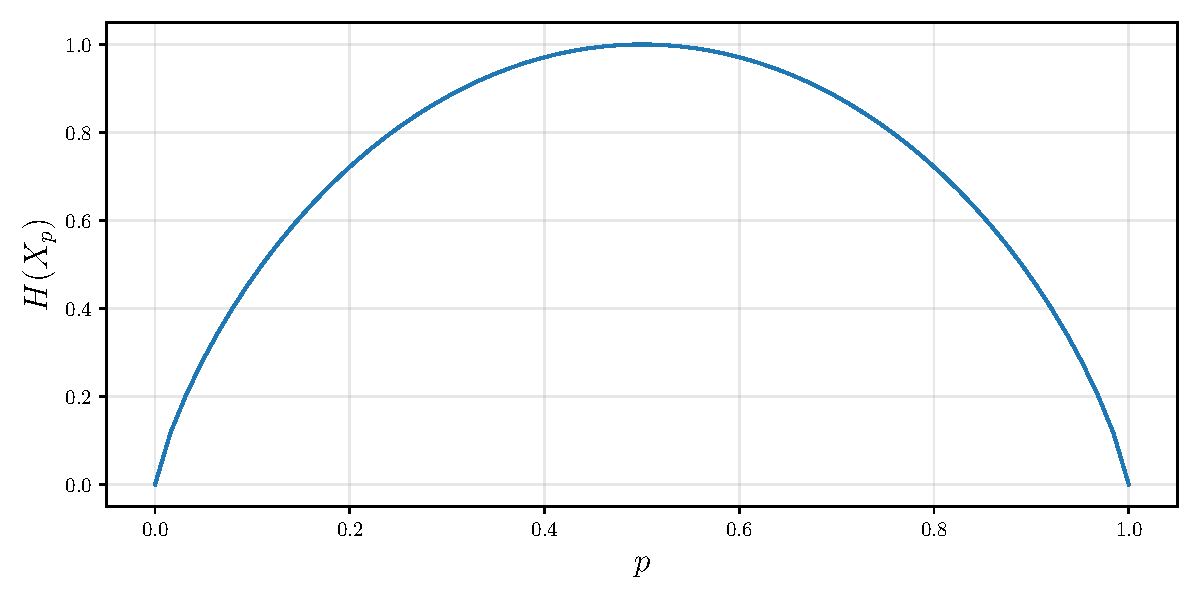
\includegraphics[width=1.0\linewidth]{../plots/entropy_weighted_coin.pdf}
        \caption{Bernoulli Rand. Variable Entropy $H(X_p)$}
        \label{fig:bernoulli-entropy}
    \end{subfigure}
    \hfill
    \begin{subfigure}[b]{0.45\textwidth}
        \centering
        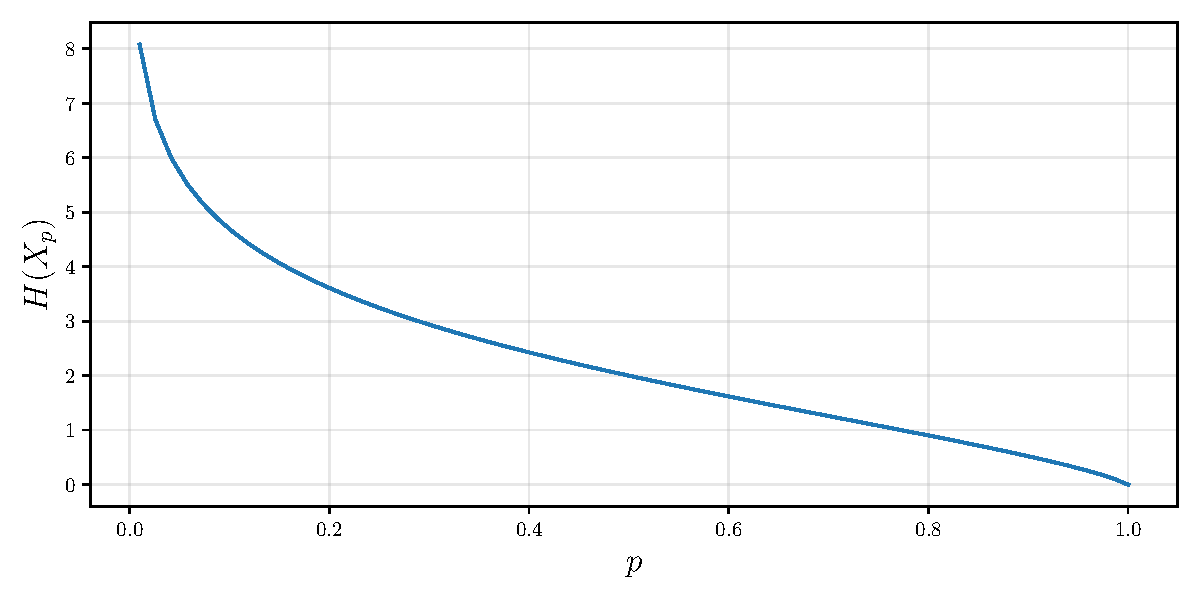
\includegraphics[width=1.0\linewidth]{../plots/entropy_geo_variable.pdf}
        \caption{Geometric Rand. Variable Entropy $H(X_p)$}
        \label{fig:geometric-entropy}
    \end{subfigure}
\end{figure}

\begin{example}[Entropy of bernoulli variable]
    Let $p \in (0, 1)$ and $X_p \sim B(1, p)$ be a weighted coin flip. \\
    We can calculate the Entropy of $X_p$: $H(X_p) = -p \log p - (1-p) \log (1-p)$. \\
    A visual inspection (see Figure \ref{fig:bernoulli-entropy}) reveals that $H(X_p)$ seems to be maximised for $p = 0.5$ and minimised for $p \in \{0, 1\}$.
    An increase in uncertainty about the result of the coin flip seems to correspond with an increase in entropy.
\end{example}

\begin{example}[Entropy of geometric variable]
    Let $p \in (0, 1)$ and $X_p \sim G(p)$ be the number of times a weighted coin is flipped, until the first head occurs.
    We will calculate the Entropy of $X_p$. It will require the two well-known series:
    \begin{align}
        \forall r \in (0, 1)&\vcentcolon \sum_{n \in \mathbb{N}_0}{r^n} = \frac{1}{1 - r} \label{series:nexpr-n}\\
        \forall r \in (0, 1)&\vcentcolon \sum_{n \in \mathbb{N}_0}{n r^n} = \frac{r}{(1 - r)^2} \label{series:expr-n}
    \end{align}
    We can now directly calculate the Entropy of $X_p$:
    \begin{align*}
        H(X_p) &= \sum_{x \in \mathbb{N}}{-p(x) \log p(x)}                                  && \text{(Def. of Entropy)}\\
        &= -\sum_{x \in \mathbb{N}}{(1-p)^{x-1} p \log\paren{(1-p)^{x-1} p}}                && \text{(Subst. in geometric mass function)} \\
        &= -\sum_{x \in \mathbb{N}}{(1-p)^{x-1} p \paren{(x-1) \log(1-p) + \log p}}         && \text{(Log rules)} \\
        &= -p \log(1-p) \sum_{x \in \mathbb{N}_{0}}\paren{(1-p)^{x} x} - p \log p \sum_{x \in \mathbb{N}_{0}}\paren{(1-p)^{x}}      && \text{(Factor out constants)} \\
        &= -p \log(1-p) \frac{1-p}{(1 - (1-p))^2} - p \log p \frac{1}{1 - (1-p)}            && \text{(Use series \ref{series:nexpr-n} and \ref{series:expr-n})}\\
        &= -p \log(1-p) \frac{1-p}{p^2} - p \log p \frac{1}{p}                              && \text{(Simplify expr.)} \\
        &= \frac{-(1-p) \log(1-p) - p \log p}{p}                                            && \text{(Simplify expr.)}
    \end{align*}
    For $p=0.5$ we get $H(X_{0.5}) = \frac{-0.5 \log 0.5 - 0.5 \log 0.5}{0.5} = -2 \log 0.5 = 2$. \\
    We can visually inspect $(0, 1) \rightarrow \mathbb{R}, p \mapsto H(X_p)$ (see Figure \ref{fig:geometric-entropy}) to get a feeling for the entropy of $X_p$.
    An increase in $p$ is linked to lower variance and more concentration of the distribution towards zero. 
    Based on the plot, that increase looks to be linked to a lower entropy and vice-versa.

    We will now find a strategy, that calculates the number of flips until the first head occurs using simple yes/no questions.
    A simple strategy is to ask "Is $X=1$?", "Is $X=2$?" and so on.
    Under this strategy, the number of questions required is exactly the value of $X$.
    Thus, the average number of questions is simply $\mathbb{E}(X_{0.5}) = \frac{1}{0.5} = 2$. 
    This matches the entropy $H(X_{0.5}) = 2$.
\end{example}

\begin{figure}[t]
    \centering
    \begin{subfigure}[b]{0.45\textwidth}
        \centering
        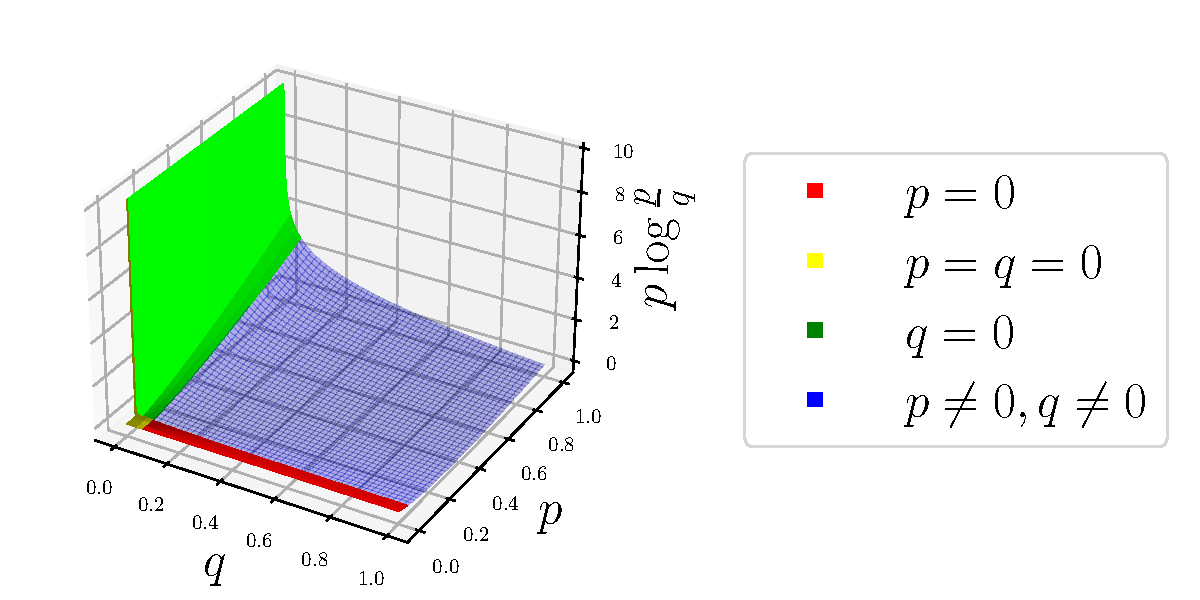
\includegraphics[width=1.0\linewidth]{../plots/pointwise_rel_entropy_continuation.pdf}
        \caption{Pointwise Relative Entropy}
        \label{fig:pointwise-rel-entropy}
    \end{subfigure}
    \hfill
    \begin{subfigure}[b]{0.45\textwidth}
        \centering
        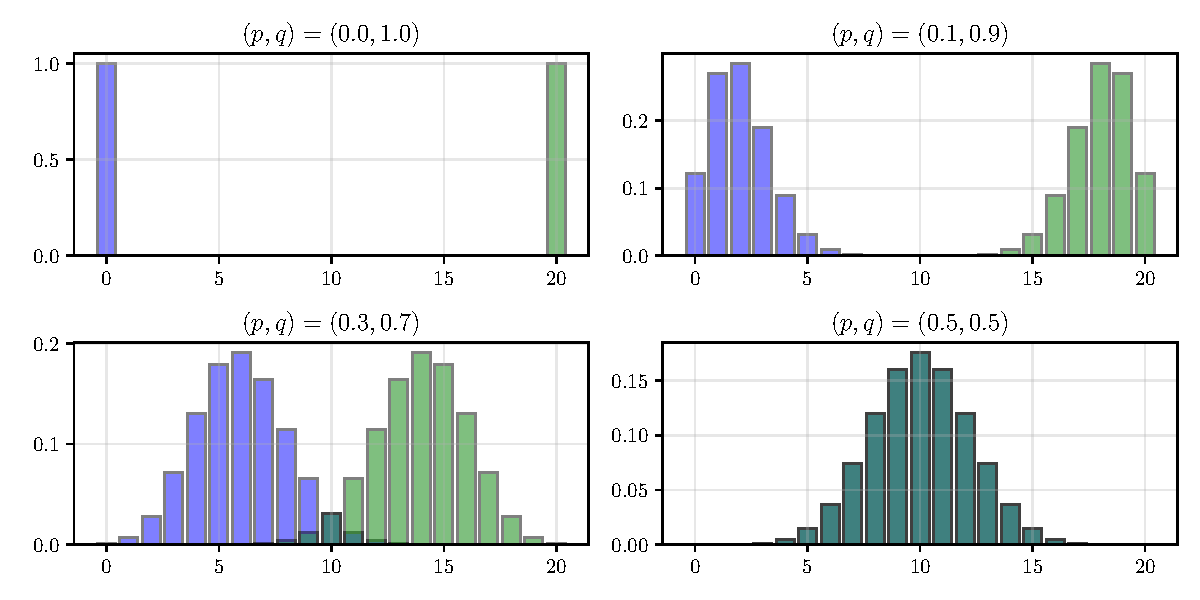
\includegraphics[width=1.0\linewidth]{../plots/relative_entropy_binomial_distributions.pdf}
        \caption{Relative Entropies of Binomial Distributions}
        \label{fig:rel-entropy-bionm-distrib}
    \end{subfigure}
\end{figure}


\begin{definition}\label{def:entropy-mutual-info-def}
    \begin{align*}
    \intertext{\noindent We define the following:}
        \textbf{Conditional Entropy:} & \quad H(X \mid Y) = -\mathbb{E}\paren{\log p_{(X \mid Y)}(X \mid Y)} \\
        \textbf{Joint Entropy:}       & \quad H(X, Y) = -\mathbb{E}\paren{\log p_{(X, Y)}(X, Y)}
    \intertext{\noindent Let $p$ and $q$ be two probability mass functions on the same set $\mathcal{Z}$. We define the following:}
        \textbf{Relative Entropy:}    & \quad D(p \| q) = \mathbb{E}_{X \sim p}\paren{\log \frac{p(X)}{q(X)}} 
            \, \text{with conventions from Remark \ref{remark:relative-entropy-conventions}}
    \intertext{(Sometimes also called KL-Divergence)}
    \intertext{\noindent Using Relative Entropy, we can define the Mutual Information between the variables $X, Y$:}
        \textbf{Mutual Information:}  & \quad I(X; Y) = D(p_{(X, Y)} \| p_X \, p_Y) \\
    \end{align*}
\end{definition}

\begin{remark} \label{remark:relative-entropy-conventions}
    We have
    \begin{align*}
        D(p \| q)   &= \mathbb{E}_{X \sim p}\paren{\log \frac{p(X)}{q(X)}}             && \text{(def.~of relative entropy)} \\
                    &= \sum_{x \in \mathcal{X}}{p(x) \log \frac{p(x)}{q(x)}}        && \text{(def.~of expected value)}
    \end{align*}
    To understand the conventions, we can look at the limit cases:
    \begin{enumerate}
        \item Case $p \in (0, 1], q = 0$: $\lim_{q \to 0^+} p \log \frac{p}{q} = \lim_{q \to 0^+} (p \log p - p \log q) = \infty$.
        \item Case $p = 0, q \in (0, 1]$: $0 \log \frac{0}{q} = 0$.
        \item Case $p = q = 0$: Case 1 logic yields $\lim_{q \to 0^+} p \log \frac{p}{q} = \infty$ and Case 2 logic yields $0 \log \frac{0}{0} = 0$. \\
            So what do we choose?
            As we want $\sum_{x \in \mathcal{X}}{p(x) \log \frac{p(x)}{q(x)}}$ to sum over $x \in \mathcal{X}, p(x) > 0$, we choose the convention $0 \log \frac{0}{0} = 0$.
    \end{enumerate}
    Figure \ref{fig:pointwise-rel-entropy} visualizes the pointwise relative entropy function $(p, q) \mapsto p \log \frac{p}{q}$.
\end{remark}

\begin{example}
    To understand the concept, we can now calculate the relative entropies for an example.
    Let $X \sim B(20, \alpha)$ and $Y \sim B(20, \beta)$ with $\paren{\alpha, \beta} \in [0, 1]^2$.
    \begin{align*}
                                 & \quad D(p_X \| p_Y) = \sum_{x = 0}^{20}{p_X(x) \log \frac{p_X(x)}{p_Y(x)}} \\
        \alpha=0, \beta=1:       & \quad D(p_X \| p_Y) = 1 \log \frac{1}{0} + 0 \log \frac{0}{1} = \infty + 0 = \infty \\
        \alpha=0.1, \beta=0.9:   & \quad D(p_X \| p_Y) \approx 50.7 \\
        \alpha=0.3, \beta=0.7:   & \quad D(p_X \| p_Y) \approx 9.8 \\
        \alpha= 0.5, \beta= 0.5: & \quad D(p_X \| p_Y) = \sum_{x = 0}^{20}{p(x) \log 1} = 0 \\
    \end{align*}
    Figure \ref{fig:rel-entropy-bionm-distrib} visualizes the two discrete distribution functions in the cases above.
    Intuitively, the more overlap the distributions have, the closer to zero the relative entropy is.
\end{example}


\subsection{Mutual Information and Chain Rules}
\begin{figure}[ht]
    \centering
    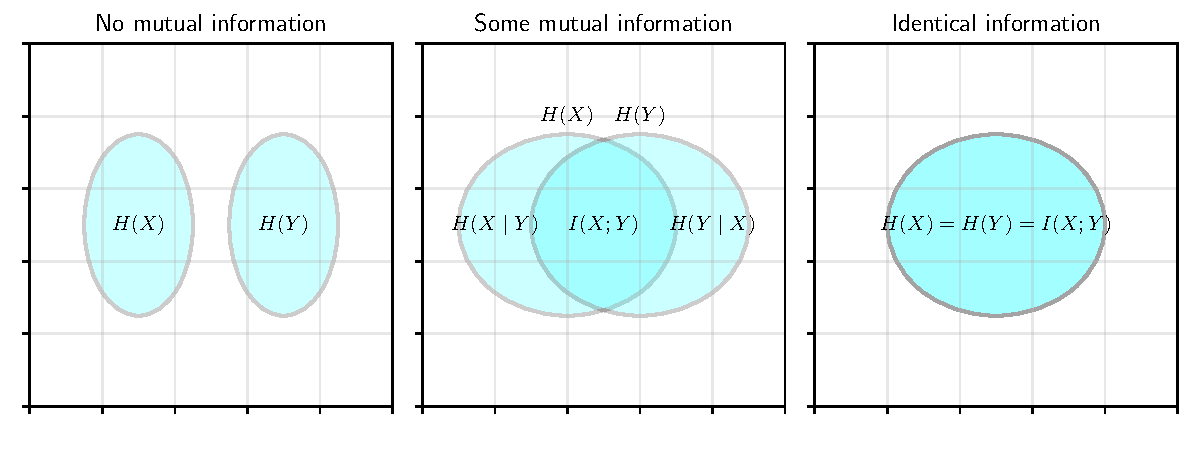
\includegraphics[width=0.9\linewidth]{../plots/entropy_mutual_info_venn_diagram.pdf}
    \caption{Relationship between Entropy, Conditional Entropy and Mutual Information}
    \label{fig:relationships-entropy-mutual-information}
\end{figure}

% Prerequisite to the next theorem.
\begin{theorem}[Chain Rule for Entropy]
    We have
    \[
        H(X, Y) = H(X) + H(Y \mid X)
    \]
\end{theorem}
\begin{proof}
    \begin{align*}
        H(X, Y) &= -\mathbb{E}\paren{\log p(X, Y)} 
        = -\mathbb{E}\paren{\log p(Y \mid X)p(X)} \\
        &= -\mathbb{E}\paren{\log p(Y \mid X)} - \mathbb{E}\paren{\log p(X)}
        = H(X) + H(Y \mid X)
    \end{align*}
\end{proof}

\begin{theorem}
    There are multiple equivalent ways to express Mutual Information (see Figure \ref{fig:relationships-entropy-mutual-information}):
    \begin{enumerate}
        \item $I(X; Y) = H(Y) - H(Y | X)$
        \item $I(X; Y) = I(Y; X)$
        \item $I(Y; X) = H(X) - H(X | Y)$
        \item $I(X; Y) = H(X) + H(Y) - H(X, Y)$
        \item $I(X; X) = H(X)$
    \end{enumerate}
\end{theorem}
\begin{proof}
    \begin{enumerate}
        \item We can use the definition of mutual information and relative entropy to obtain:
            \begin{align*}
                I(X; Y) &= D(p_{(X, Y)} \| p_X p_Y)                                                                                         && \text{(by def.~of mutual info.)}\\
                        &= \mathbb{E}_{p_{(X, Y)}}\paren{\log \frac{p_{(X, Y)}(X, Y)}{p_X(X)p_Y(Y)}}                                        && \text{(by def.~relative entropy)} \\
                        &= \mathbb{E}_{p_{(X, Y)}}\paren{\log \frac{p_X(X)p_{(Y \mid X)}{(Y \mid X)}}{p_X(X)p_Y(Y)}}                        && \text{(using cond.~probability)} \\
                        &= \mathbb{E}_{p_{(X, Y)}}\paren{\log \frac{p_{(Y \mid X)}(Y \mid X)}{p_Y(Y)}}                                      && \text{(simplify fraction)} \\
                        &= \mathbb{E}_{p_{(X, Y)}}\paren{\log p_{(Y \mid X)}(Y \mid X)} - \mathbb{E}_{p_{(X, Y)}}\paren{\log p_Y(Y)}        && \text{(simplify logarithm)} \\
                        &= -H(Y \mid X) + H(Y)                                                                                              && \text{(by def.~of entropy)}
            \end{align*}
        \item The definition of mutual information yields:
            \begin{align*}
                I(X; Y) &= D(P[X = x, Y = y] \| P[X = x]P[Y = y])       && \text{(by def.~of mutual info.)} \\
                        &= D(P[Y = y, X = x] \| P[Y = y]P[X = x]) = I(Y; X)
            \end{align*}
        \item Follows directly from 1 and 2.
        \item \begin{align*}
                I(X; Y) &= H(Y) - H(Y \mid X)               && \text{(by 1)} \\
                        &= H(Y) - \paren{H(X, Y) - H(X)}    && \text{(chain rule)} \\
                        &= H(X) + H(Y) - H(X, Y)
            \end{align*}
        \item Using the Defintion we get $H(X \mid X) = 0$. Using 1 we get $I(X; X) = H(X) - H(X \mid X) = H(X)$.
    \end{enumerate}
\end{proof}

\begin{definition}\label{def:conditional-entropy-mutual}
    Let $p$ and $q$ be probability mass functions on $\mathcal{X} \times \mathcal{Y}$.
    We define the following:
    \begin{align*}
        \textbf{Conditional Relative Entropy:}    & \quad D(p_{Y \mid X} \| q_{Y \mid X}) \\
        &= \mathbb{E}_{X \sim p_X} D(p(Y \mid X) \| q(Y \mid X)) \\
        &= \sum_{x \in \mathcal{X}}{p(x) D(p(y \mid x) \| q(y \mid x))} \\
        &= \mathbb{E}_{(X, Y) \sim p(x, y)}\paren{\log \frac{p(Y \mid X)}{q(Y \mid X)}} \\
        &= \sum_{(x, y) \injoint}{p(x, y) \log \frac{p(y \mid x)}{q(y \mid x)}} \\
        \textbf{Conditional Mutual Information:}  & \quad I(X; Y \mid Z) 
        = H(X \mid Z) - H(X \mid Y, Z)
    \end{align*}
\end{definition}

\begin{example}
    The Conditional Relative Entropy can be illustrated using a Christmas example: \\
    Let $\Omega = \{1, \cdots, 12\}$, $\mathds{P}$ uniformly distributed, \\
    $\mathcal{X} = \{\textbf{JANUARY}, \cdots, \textbf{DECEMBER}\}$ and
    $\mathcal{Y} = \{0, 1\}$. \\
    Our variable $X$ gives us the month of the year: \\
    We define it as $X: \Omega \rightarrow \mathcal{X}, \omega \mapsto \textbf{the corresponding month}$. \\
    Our variable $Y$ answers the question "Is Christmas Advent?": \\
    We define it as $Y: \Omega \rightarrow \mathcal{Y}, \omega \mapsto \mathds{1}_{\{\textbf{NOVEMBER}, \textbf{DECEMBER}\}}(\omega)$. \\
    We have lived on earth our entire lives. Our model of reality $p$ is correct! \\
    We define it as
    \[
        p(Y = 1 \mid x) = \begin{cases}
			1, & \text{if $x \in \{\textbf{NOVEMBER}, \textbf{DECEMBER}\}$} \\
            0, & \text{otherwise}
		\end{cases}
    \]
    The alien \textit{ET} visits earth. He sees the Christmas trees in January and assumes Advent continues into January.
    In November and December, he is uncertain too. His model of reality $q$ is not correct! \\
    We define it as 
    \[
        q(Y = 1 \mid x) = \begin{cases}
			0.5, & \text{if $x \in \{\textbf{NOVEMBER}, \textbf{DECEMBER}, \textbf{JANUARY}\}$} \\
            0, & \text{otherwise}
		\end{cases}
    \]
    Let us calculate the individual relative entropies:
    \begin{enumerate}
        \item $D(p(y \mid \textbf{NOV.}) \| q(y \mid \textbf{NOV.})) = 0 + 1 \log \frac{1}{0.5} = 1$
        \item $D(p(y \mid \textbf{DEC.}) \| q(y \mid \textbf{DEC.})) = 0 + 1 \log \frac{1}{0.5} = 1$
        \item $D(p(y \mid \textbf{JAN.}) \| q(y \mid \textbf{JAN.})) = 1 \log \frac{1}{0.5} + 0 = 1$
        \item Otherwise: $D(p(y \mid x) \| q(y \mid x)) = 0$
    \end{enumerate}
    We can now calculate the Conditional Relative Entropy:
    \begin{align*}
        D(p_{Y \mid X} \| q_{Y \mid X}) &= \sum_{x \in \mathcal{X}}{p_X(x) D(p(y \mid x) \| q(y \mid x))} \\
        &= \frac{1}{12} \paren{1 + 1 + 1} = \frac{3}{12} = 0.25
    \end{align*}
    So the expression calculates how much of an error \textit{ET} makes per month, on average.
\end{example}

% TODO: Explain all of these notations first.

\begin{theorem}[Chain Rules] \label{theorem:chain-rules}
    Let $n \in \mathbb{N}, n \ge 2$, $(X_1, \cdots, X_n) \sim p(x_1, \cdots, x_n)$ and $Y$ a random variable.
    The following statements about Entropy and Mutual Information are called Chain Rules:
    \begin{enumerate}
        \item
            \[
                H(X_1, \cdots, X_n) = \sum_{i=1}^{n}{H(X_i \mid X_{i-1}, \cdots, X_1)}
            \]
        \item
            \[
                D(p(x) \| q(x)) = D(p(x \mid y) \| q(x \mid y)) + D(p(y) \| q(y))
            \]
        \item
            \[
                I(X_1, \cdots, X_n; Y) = \sum_{i=1}^{n}{I(X_i; Y \mid X_{i-1}, \cdots, X_1)}
            \]
    \end{enumerate}
\end{theorem}
\begin{proof}
    \begin{enumerate}
        \item 
            Prove this result using induction by $n$. \\
            Base case $n = 2$:
            \begin{align*}
                H(X_1, X_2) &= -\mathbb{E}\paren{\log p(X_1, X_2)} \\
                &= -\mathbb{E}\paren{\log p(X_2 \mid X_1)p(X_1)} \\
                &= -\mathbb{E}\paren{\log p(X_2 \mid X_1)} + -\mathbb{E}\paren{\log p(X_1)} \\
                &= H(X_1) + H(X_2 \mid X_1)
            \end{align*}
            Assume the theorem holds for $n - 1$. Induction case $n - 1$ to $n$:
            \begin{align*}
                H(X_1, \cdots, H_n) &= H(X_n | X_1, \cdots, H_{n-1}) + H(X_1, \cdots, H_{n-1})          && \text{(apply base case)} \\
                &= H(X_n | X_1, \cdots, H_{n-1}) + \sum_{i=1}^{n-1}{H(X_i \mid X_{i-1}, \cdots, X_1)}   && \text{(induction hypothesis)}
            \end{align*}

        \item
            \begin{align*}
                D(p(x) \| q(x)) &= \sum_{(x, y) \injoint}{p(x, y) \frac{p(x)}{q(x)}}
                = \sum_{(x, y) \injoint}{p(x, y) \frac{p(x)}{q(x)}}
                = \sum_{(x, y) \injoint}{p(x, y) \frac{p(x \mid y)p(y)}{q(x \mid y)p(y)}} \\
                &= \sum_{(x, y) \injoint}{p(x, y) \frac{p(x \mid y)}{q(x \mid y)}} + \sum_{(x, y) \injoint}{p(x, y) \frac{p(y)}{p(y)}} \\
                &= D(p(x \mid y) \| q(x \mid y)) + D(p(y) \| q(y))
            \end{align*}
        
        \item
            \begin{align*}
                I(X_1, \cdots, X_n; Y) &= H(X_1, \cdots, X_n) - H(X_1, \cdots, X_n \mid Y) \\
                &= \sum_{i=1}^{n}{H(X_i \mid X_{i-1}, \cdots, X_1)} + \sum_{i=1}^{n}{H(X_i \mid X_{i-1}, \cdots, X_1, Y)} \\
                &= \sum_{i=1}^{n}{I(X_i; Y \mid X_{i-1}, \cdots, X_1)}
            \end{align*}

    \end{enumerate}
\end{proof}

% TODO: Definition of relative entropy correctly uses E_p everywhere instead of E.
